
\documentclass[11pt]{amsart}
\usepackage{geometry} % see geometry.pdf on how to lay out the page. There's lots.
\usepackage{graphicx}
\geometry{a4paper} % or letter or a5paper or ... etc
% \geometry{landscape} % rotated page geometry

% See the ``Article customise'' template for come common customisations

\title{PBHLT 7115: Causal Methods for Public Health }
\author{Homework 1}
\date{} % delete this line to display the current date

%%% BEGIN DOCUMENT
\begin{document}

\maketitle
%\tableofcontents

\section{1. Use Dagitty to reproduce the following DAG}

\begin{figure}[h]
\centering
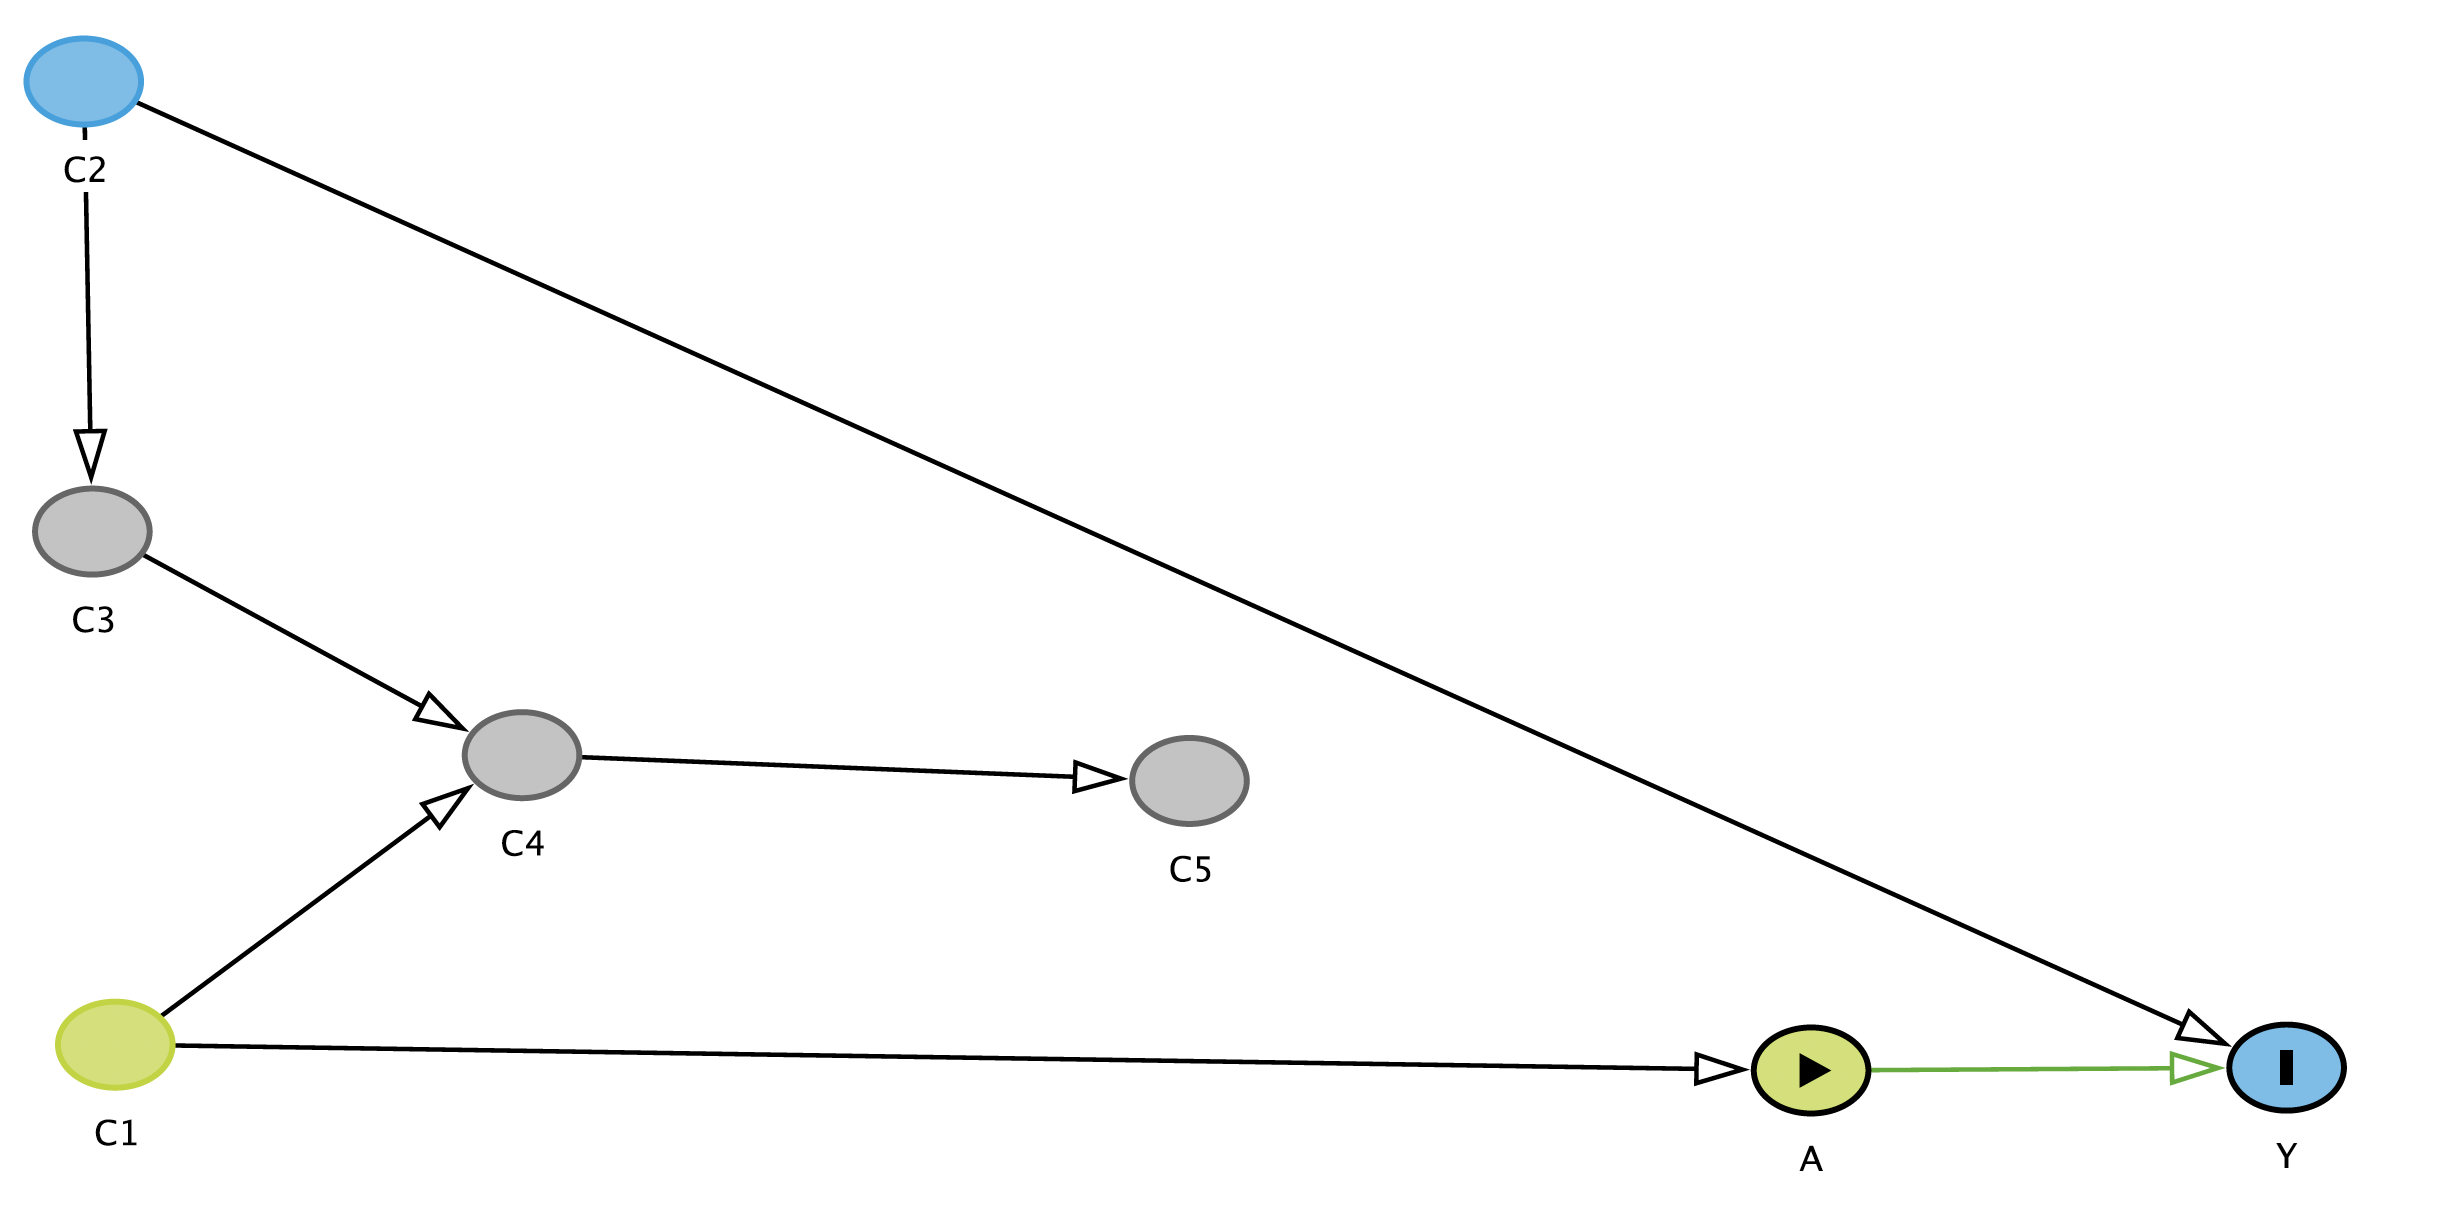
\includegraphics[scale=0.4]{DAG.png}
\end{figure}


\newpage

\subsection{What is the minimal sufficient adjustment set(s)?}\

(Hint: remember it is possible for the minimal sufficient adjustment set to be $\emptyset$)

\vspace{4cm}

\subsection{Show that adjusting C4 opens a backdoor path (red lines.) }\

\vspace{4cm}

\subsection{if you adjust for C4, list all the minimal sufficient adjustment sets including C4.}\

i.e., What are the minimal sufficient adjustment sets containing C4 for estimating the total effect of A on Y?


\vspace{4cm}

\subsection{Is the set {C1, C2, C3}  a sufficient adjustment set? Why? }

\end{document}